\documentclass[a4paper,12pt]{article} 

% First, we usually want to set the margins of our document. For this we use the package geometry.
\usepackage[top = 2.5cm, bottom = 2.5cm, left = 2.5cm, right = 2.5cm]{geometry} 
\usepackage[T1]{fontenc}
\usepackage[utf8]{inputenc}

% The following two packages - multirow and booktabs - are needed to create nice looking tables.
\usepackage{multirow} % Multirow is for tables with multiple rows within one cell.
\usepackage{booktabs} % For even nicer tables.

% As we usually want to include some plots (.pdf files) we need a package for that.
\usepackage{graphicx} 

% The default setting of LaTeX is to indent new paragraphs. This is useful for articles. But not really nice for homework problem sets. The following command sets the indent to 0.
\usepackage{setspace}
\setlength{\parindent}{0in}

% Package to place figures where you want them.
\usepackage{float}

% The fancyhdr package let's us create nice headers.
\usepackage{fancyhdr}

\usepackage{amsmath,amsthm,circuitikz,colortbl,karnaugh-map,caption}

% To make our document nice we want a header and number the pages in the footer.

\pagestyle{fancy} % With this command we can customize the header style.

\fancyhf{} % This makes sure we do not have other information in our header or footer.

\lhead{\footnotesize Digital Logic(H): Theory Assignment 4}% \lhead puts text in the top left corner. \footnotesize sets our font to a smaller size.

%\rhead works just like \lhead (you can also use \chead)
\rhead{\footnotesize Mengxuan Wu} %<---- Fill in your lastnames.

% Similar commands work for the footer (\lfoot, \cfoot and \rfoot).
% We want to put our page number in the center.
\cfoot{\footnotesize \thepage} 

\begin{document}

\thispagestyle{empty} % This command disables the header on the first page. 

\begin{tabular}{p{15.5cm}}
{\large \bf Digital Logic(H)} \\
Southern University of Science and Technology \\ Mengxuan Wu \\ 12212006 \\
\hline
\\
\end{tabular}

\vspace*{0.3cm} %add some vertical space in between the line and our title.

\begin{center}
	{\Large \bf Theory Assignment 4}
	\vspace{2mm}

	{\bf Mengxuan Wu}
		
\end{center}  

\vspace{0.4cm}

\section*{1.}

\textbf{Function Table:}

\begin{center}
	\begin{tabular}{ccccccl}
		\toprule
		$S_1$ & $S_0$ & $Q_3^+$ & $Q_2^+$ & $Q_1^+$ & $Q_0^+$ & Operation \\
		\midrule
		0 & 0 & $Q_3$ & $Q_2$ & $Q_1$ & $Q_0$ & No Change \\
		0 & 1 & $Q_3'$ & $Q_2'$ & $Q_1'$ & $Q_0'$ & Complement the four outputs \\
		1 & 0 & 0 & 0 & 0 & 0 & Clear register to 0 \\
		1 & 1 & $D_3$ & $D_2$ & $D_1$ & $D_0$ & Load parallel data \\
		\bottomrule
	\end{tabular}
\end{center}

\textbf{Logic Diagram:}

\begin{center}
	\resizebox{\linewidth}{!}{
		\begin{circuitikz}
			\tikzset{myflipflop D/.style={flipflop,flipflop def={t1=D, t3={\texttt{CLK}}, t4=Q, t6=Q, n4=1, c3=1}}}
			\tikzset{4to1mux/.style={muxdemux, muxdemux def={Lh=2, Rh=4, NL=1, NT=0, NR=4, NB=2, w=2, square pins=1}}}
			\draw (-0.85,-4) node[4to1mux, rotate=-90] (MUX1) {\rotatebox{90}{MUX}};
			\draw (0,0) node[myflipflop D, rotate=90] (DFF1) {\rotatebox{-90}{$Q_3$}};
			\draw (DFF1.pin 6) -- ++(0,0.75) node[circ]{} -- ++(2.4,0) -- ++(0,-7) -| (MUX1.rpin 4);
			\draw (DFF1.pin 6) -- ++(0,1.5) node[above] {$Q_3$};
			\draw (DFF1.pin 4) -- ++(0,0.25) -- ++(1.4,0) -- ++(0,-7) -| (MUX1.rpin 3);
			\draw (MUX1.rpin 2) -- ++(0,-1.5) node[below] {0};
			\draw (MUX1.rpin 1) -- ++(0,-1.5) node[below] {$D_3$};
			\draw (MUX1.lpin 1) -- (DFF1.pin 1);
			\draw (MUX1.brpin 4) node [above, yshift=-3] {$I_0$};
			\draw (MUX1.brpin 3) node [above, yshift=-3] {$I_1$};
			\draw (MUX1.brpin 2) node [above, yshift=-3] {$I_2$};
			\draw (MUX1.brpin 1) node [above, yshift=-3] {$I_3$};
	
			\draw (4.15,-4) node[4to1mux, rotate=-90] (MUX2) {\rotatebox{90}{MUX}};
			\draw (5,0) node[myflipflop D, rotate=90] (DFF2) {\rotatebox{-90}{$Q_2$}};
			\draw (DFF2.pin 6) -- ++(0,0.75) node[circ]{} -- ++(2.4,0) -- ++(0,-7) -| (MUX2.rpin 4);
			\draw (DFF2.pin 6) -- ++(0,1.5) node[above] {$Q_2$};
			\draw (DFF2.pin 4) -- ++(0,0.25) -- ++(1.4,0) -- ++(0,-7) -| (MUX2.rpin 3);
			\draw (MUX2.rpin 2) -- ++(0,-1.5) node[below] {0};
			\draw (MUX2.rpin 1) -- ++(0,-1.5) node[below] {$D_2$};
			\draw (MUX2.lpin 1) -- (DFF2.pin 1);
			\draw (MUX2.brpin 4) node [above, yshift=-3] {$I_0$};
			\draw (MUX2.brpin 3) node [above, yshift=-3] {$I_1$};
			\draw (MUX2.brpin 2) node [above, yshift=-3] {$I_2$};
			\draw (MUX2.brpin 1) node [above, yshift=-3] {$I_3$};
	
			\draw (9.15,-4) node[4to1mux, rotate=-90] (MUX3) {\rotatebox{90}{MUX}};
			\draw (10,0) node[myflipflop D, rotate=90] (DFF3) {\rotatebox{-90}{$Q_1$}};
			\draw (DFF3.pin 6) -- ++(0,0.75) node[circ]{} -- ++(2.4,0) -- ++(0,-7) -| (MUX3.rpin 4);
			\draw (DFF3.pin 6) -- ++(0,1.5) node[above] {$Q_1$};
			\draw (DFF3.pin 4) -- ++(0,0.25) -- ++(1.4,0) -- ++(0,-7) -| (MUX3.rpin 3);
			\draw (MUX3.rpin 2) -- ++(0,-1.5) node[below] {0};
			\draw (MUX3.rpin 1) -- ++(0,-1.5) node[below] {$D_1$};
			\draw (MUX3.lpin 1) -- (DFF3.pin 1);
			\draw (MUX3.brpin 4) node [above, yshift=-3] {$I_0$};
			\draw (MUX3.brpin 3) node [above, yshift=-3] {$I_1$};
			\draw (MUX3.brpin 2) node [above, yshift=-3] {$I_2$};
			\draw (MUX3.brpin 1) node [above, yshift=-3] {$I_3$};
	
			\draw (14.15,-4) node[4to1mux, rotate=-90] (MUX4) {\rotatebox{90}{MUX}};
			\draw (15,0) node[myflipflop D, rotate=90] (DFF4) {\rotatebox{-90}{$Q_0$}};
			\draw (DFF4.pin 6) -- ++(0,0.75) node[circ]{} -- ++(2.4,0) -- ++(0,-7) -| (MUX4.rpin 4);
			\draw (DFF4.pin 6) -- ++(0,1.5) node[above] {$Q_0$};
			\draw (DFF4.pin 4) -- ++(0,0.25) -- ++(1.4,0) -- ++(0,-7) -| (MUX4.rpin 3);
			\draw (MUX4.rpin 2) -- ++(0,-1.5) node[below] {0};
			\draw (MUX4.rpin 1) -- ++(0,-1.5) node[below] {$D_0$};
			\draw (MUX4.lpin 1) -- (DFF4.pin 1);
			\draw (MUX4.brpin 4) node [above, yshift=-3] {$I_0$};
			\draw (MUX4.brpin 3) node [above, yshift=-3] {$I_1$};
			\draw (MUX4.brpin 2) node [above, yshift=-3] {$I_2$};
			\draw (MUX4.brpin 1) node [above, yshift=-3] {$I_3$};
	
			\draw (-4,-1.5) node[left] (clk) {$clk$};
			\draw (clk) -- (clk-|DFF1.pin 3) node[circ]{} -- (DFF1.pin 3);
			\draw (clk) -- (clk-|DFF2.pin 3) node[circ]{} -- (DFF2.pin 3);
			\draw (clk) -- (clk-|DFF3.pin 3) node[circ]{} -- (DFF3.pin 3);
			\draw (clk) -| (DFF4.pin 3);
	
			\draw (-4,-2) node[left] (s1) {$S_1$};
			\draw (s1) -- (s1-|MUX1.bpin 1) node[circ]{} -- (MUX1.bpin 1);
			\draw (s1) -- (s1-|MUX2.bpin 1) node[circ]{} -- (MUX2.bpin 1);
			\draw (s1) -- (s1-|MUX3.bpin 1) node[circ]{} -- (MUX3.bpin 1);
			\draw (s1) -| (MUX4.bpin 1);
	
			\draw (-4,-2.5) node[left] (s0) {$S_0$};
			\draw (MUX1.bpin 2) -- ++(-0.25,0) node (div1) {} -- (s0-|div1) node[circ]{} -- (s0);
			\draw (MUX2.bpin 2) -- ++(-0.25,0) node (div2) {} -- (s0-|div2) node[circ]{} -- (s0);
			\draw (MUX3.bpin 2) -- ++(-0.25,0) node (div3) {} -- (s0-|div3) node[circ]{} -- (s0);
			\draw (MUX4.bpin 2) -- ++(-0.25,0) node (div4) {} |- (s0);
		\end{circuitikz}
	}
\end{center}

\newpage
\section*{2.}

With 7 possible states, we start with 3 flip-flops. 
\begin{center}
	\begin{tabular}{cccc}
		\toprule
		$Z$ & $Q_2$ & $Q_1$ & $Q_0$ \\
		\midrule
		\rowcolor{green!20}
		0 & 1 & 0 & 1 \\
		1 & 0 & 1 & 0 \\
		\rowcolor{green!20}
		1 & 1 & 0 & 1 \\
		1 & 1 & 1 & 0 \\
		\rowcolor{red!20}
		1 & 1 & 1 & 1 \\
		\rowcolor{red!20}
		0 & 1 & 1 & 1 \\
		1 & 0 & 1 & 1 \\
		\bottomrule
	\end{tabular}
\end{center}

However, there are identical states with different outputs. 
We can add another flip-flop to make the circuit work.
\begin{center}
	\begin{tabular}{ccccc}
		\toprule
		$Z$ & $Q_3$ & $Q_2$ & $Q_1$ & $Q_0$ \\
		\midrule
		0 & 1 & 0 & 1 & 1 \\
		1 & 0 & 1 & 0 & 1 \\
		1 & 1 & 0 & 1 & 0 \\
		1 & 1 & 1 & 0 & 1 \\
		1 & 1 & 1 & 1 & 0 \\
		0 & 1 & 1 & 1 & 1 \\
		1 & 0 & 1 & 1 & 1 \\
		\bottomrule
	\end{tabular}
\end{center}

Now there are no identical states with different outputs.

\textbf{Karnaugh Maps:}
\begin{center}
	\begin{karnaugh-map}(label=corner)[4][4][1][$Q_1Q_0$][$Q_3Q_2$]
		\minterms{5,7,10,13,14}
		\maxterms{11,15}
		\autoterms[X]
		\implicant{0}{6}
		\implicant{0}{9}
		\implicantedge{0}{8}{2}{10}
	\end{karnaugh-map}
\end{center}

\textbf{Simplified Boolean Expression:}
\begin{equation*}
	Z = Q_0' + Q_1' + Q_3'
\end{equation*}

\newpage
\textbf{Logic Diagram:}
\begin{center}
	\begin{circuitikz}
		\tikzset{myflipflop D/.style={flipflop,flipflop def={t1=D, t3={\texttt{CLK}}, t4=Q, t6=Q, n4=1, c3=1}}}
		\draw (0,0) node[myflipflop D] (DFF1) {$Q_3$};
		\draw (3.5,0) node[myflipflop D] (DFF2) {$Q_2$};
		\draw (7,0) node[myflipflop D] (DFF3) {$Q_1$};
		\draw (10.5,0) node[myflipflop D] (DFF4) {$Q_0$};
		\draw (-1,-2.5) node[or port, rotate=180, number inputs=3] (OR1) {};
		\draw (-3,-1.5) node[left] (clk) {$clk$};

		\draw (DFF1.pin 6) -- (DFF2.pin 1);
		\draw (DFF2.pin 6) -- (DFF3.pin 1);
		\draw (DFF3.pin 6) -- (DFF4.pin 1);
		\draw (DFF4.pin 6) -- ++(1.5,0);
		\draw (DFF1.pin 4) |- (OR1.in 3);
		\draw (DFF3.pin 4) |- (OR1.in 2);
		\draw (DFF4.pin 4) |- (OR1.in 1);
		\draw (OR1.out) -- ++(-0.5,0) |- (DFF1.pin 1);
		\draw (DFF1.pin 3) -- (DFF1.pin 3|-clk) node[circ]{} -- (clk);
		\draw (DFF2.pin 3) -- (DFF2.pin 3|-clk) node[circ]{} -- (clk);
		\draw (DFF3.pin 3) -- (DFF3.pin 3|-clk) node[circ]{} -- (clk);
		\draw (DFF4.pin 3) |- (clk);
	\end{circuitikz}
\end{center}

\section*{3.}

\textbf{State Table:}

\begin{center}
	\begin{tabular}{cccccccccccc}
		\toprule
		\multicolumn{4}{c}{Current State} & \multicolumn{4}{c}{Next State} \\
		\cmidrule(lr){1-4} \cmidrule(lr){5-8}
		$Q_3$ & $Q_2$ & $Q_1$ & $Q_0$ & $Q_3^+$ & $Q_2^+$ & $Q_1^+$ & $Q_0^+$ \\
		\midrule
		0 & 0 & 0 & 0 & 0 & 0 & 1 & 0 \\ 
        0 & 0 & 0 & 1 & 0 & 0 & 1 & 0 \\ 
        0 & 0 & 1 & 0 & 0 & 1 & 1 & 0 \\ 
        0 & 0 & 1 & 1 & 0 & 0 & 1 & 0 \\ 
        0 & 1 & 0 & 0 & 0 & 0 & 1 & 0 \\ 
        0 & 1 & 0 & 1 & 0 & 0 & 1 & 0 \\ 
        0 & 1 & 1 & 0 & 1 & 0 & 0 & 1 \\ 
        0 & 1 & 1 & 1 & 0 & 0 & 1 & 0 \\ 
        1 & 0 & 0 & 0 & 1 & 1 & 0 & 0 \\ 
        1 & 0 & 0 & 1 & 1 & 0 & 0 & 0 \\ 
        1 & 0 & 1 & 0 & 0 & 0 & 1 & 0 \\ 
        1 & 0 & 1 & 1 & 0 & 0 & 1 & 0 \\ 
        1 & 1 & 0 & 0 & 1 & 1 & 0 & 1 \\ 
        1 & 1 & 0 & 1 & 0 & 0 & 1 & 0 \\ 
        1 & 1 & 1 & 0 & 0 & 0 & 1 & 0 \\ 
        1 & 1 & 1 & 1 & 0 & 0 & 1 & 0 \\ 
		\bottomrule
	\end{tabular}
\end{center}

\newpage
\textbf{Karnaugh Maps:}

\begin{figure}[H]
	\begin{minipage}{0.5\linewidth}
		\centering
		\begin{karnaugh-map}(label=corner)[4][4][1][$Q_1Q_0$][$Q_3Q_2$]
			\minterms{6,8,9,12}
			\maxterms{0,1,2,3,4,5,7,10,11,13,14,15}
			\implicant{6}{6}
			\implicant{12}{8}
			\implicant{8}{9}
		\end{karnaugh-map}
		\caption*{$D_3$}
	\end{minipage}
	\begin{minipage}{0.5\linewidth}
		\centering
		\begin{karnaugh-map}(label=corner)[4][4][1][$Q_1Q_0$][$Q_3Q_2$]
			\minterms{2,8,12}
			\maxterms{0,1,3,4,5,6,7,9,10,11,13,14,15}
			\implicant{2}{2}
			\implicant{12}{8}
		\end{karnaugh-map}
		\caption*{$D_2$}
	\end{minipage}
\end{figure}

\begin{figure}[H]
	\begin{minipage}{0.5\linewidth}
		\centering
		\begin{karnaugh-map}(label=corner)[4][4][1][$Q_1Q_0$][$Q_3Q_2$]
			\minterms{0,1,2,3,4,5,7,10,11,13,14,15}
			\maxterms{6,8,9,12}
			\implicant{0}{2}
			\implicant{0}{5}
			\implicant{5}{15}
			\implicant{15}{10}
		\end{karnaugh-map}
		\caption*{$D_1$}
	\end{minipage}
	\begin{minipage}{0.5\linewidth}
		\centering
		\begin{karnaugh-map}(label=corner)[4][4][1][$Q_1Q_0$][$Q_3Q_2$]
			\minterms{6,12}
			\maxterms{0,1,2,3,4,5,7,8,9,10,11,13,14,15}
			\implicant{6}{6}
			\implicant{12}{12}
		\end{karnaugh-map}
		\caption*{$D_0$}
	\end{minipage}
\end{figure}

\textbf{Simplified Boolean Expression:}

\begin{align*}
	D_3 =& Q_3Q_1'Q_0' + Q_3Q_2'Q_1' + Q_3'Q_2Q_1Q_0' \\
	D_2 =& Q_3Q_1'Q_0' + Q_3'Q_2'Q_1Q_0' \\
	D_1 =& Q_3'Q_2' + Q_3'Q_1' + Q_2Q_0 + Q_3Q_1 \\
	D_0 =& Q_3Q_2Q_1'Q_0' + Q_3'Q_2Q_1Q_0'
\end{align*}

\newpage
\textbf{Logic Diagram:}

\begin{center}
	\resizebox{\linewidth}{!}{
		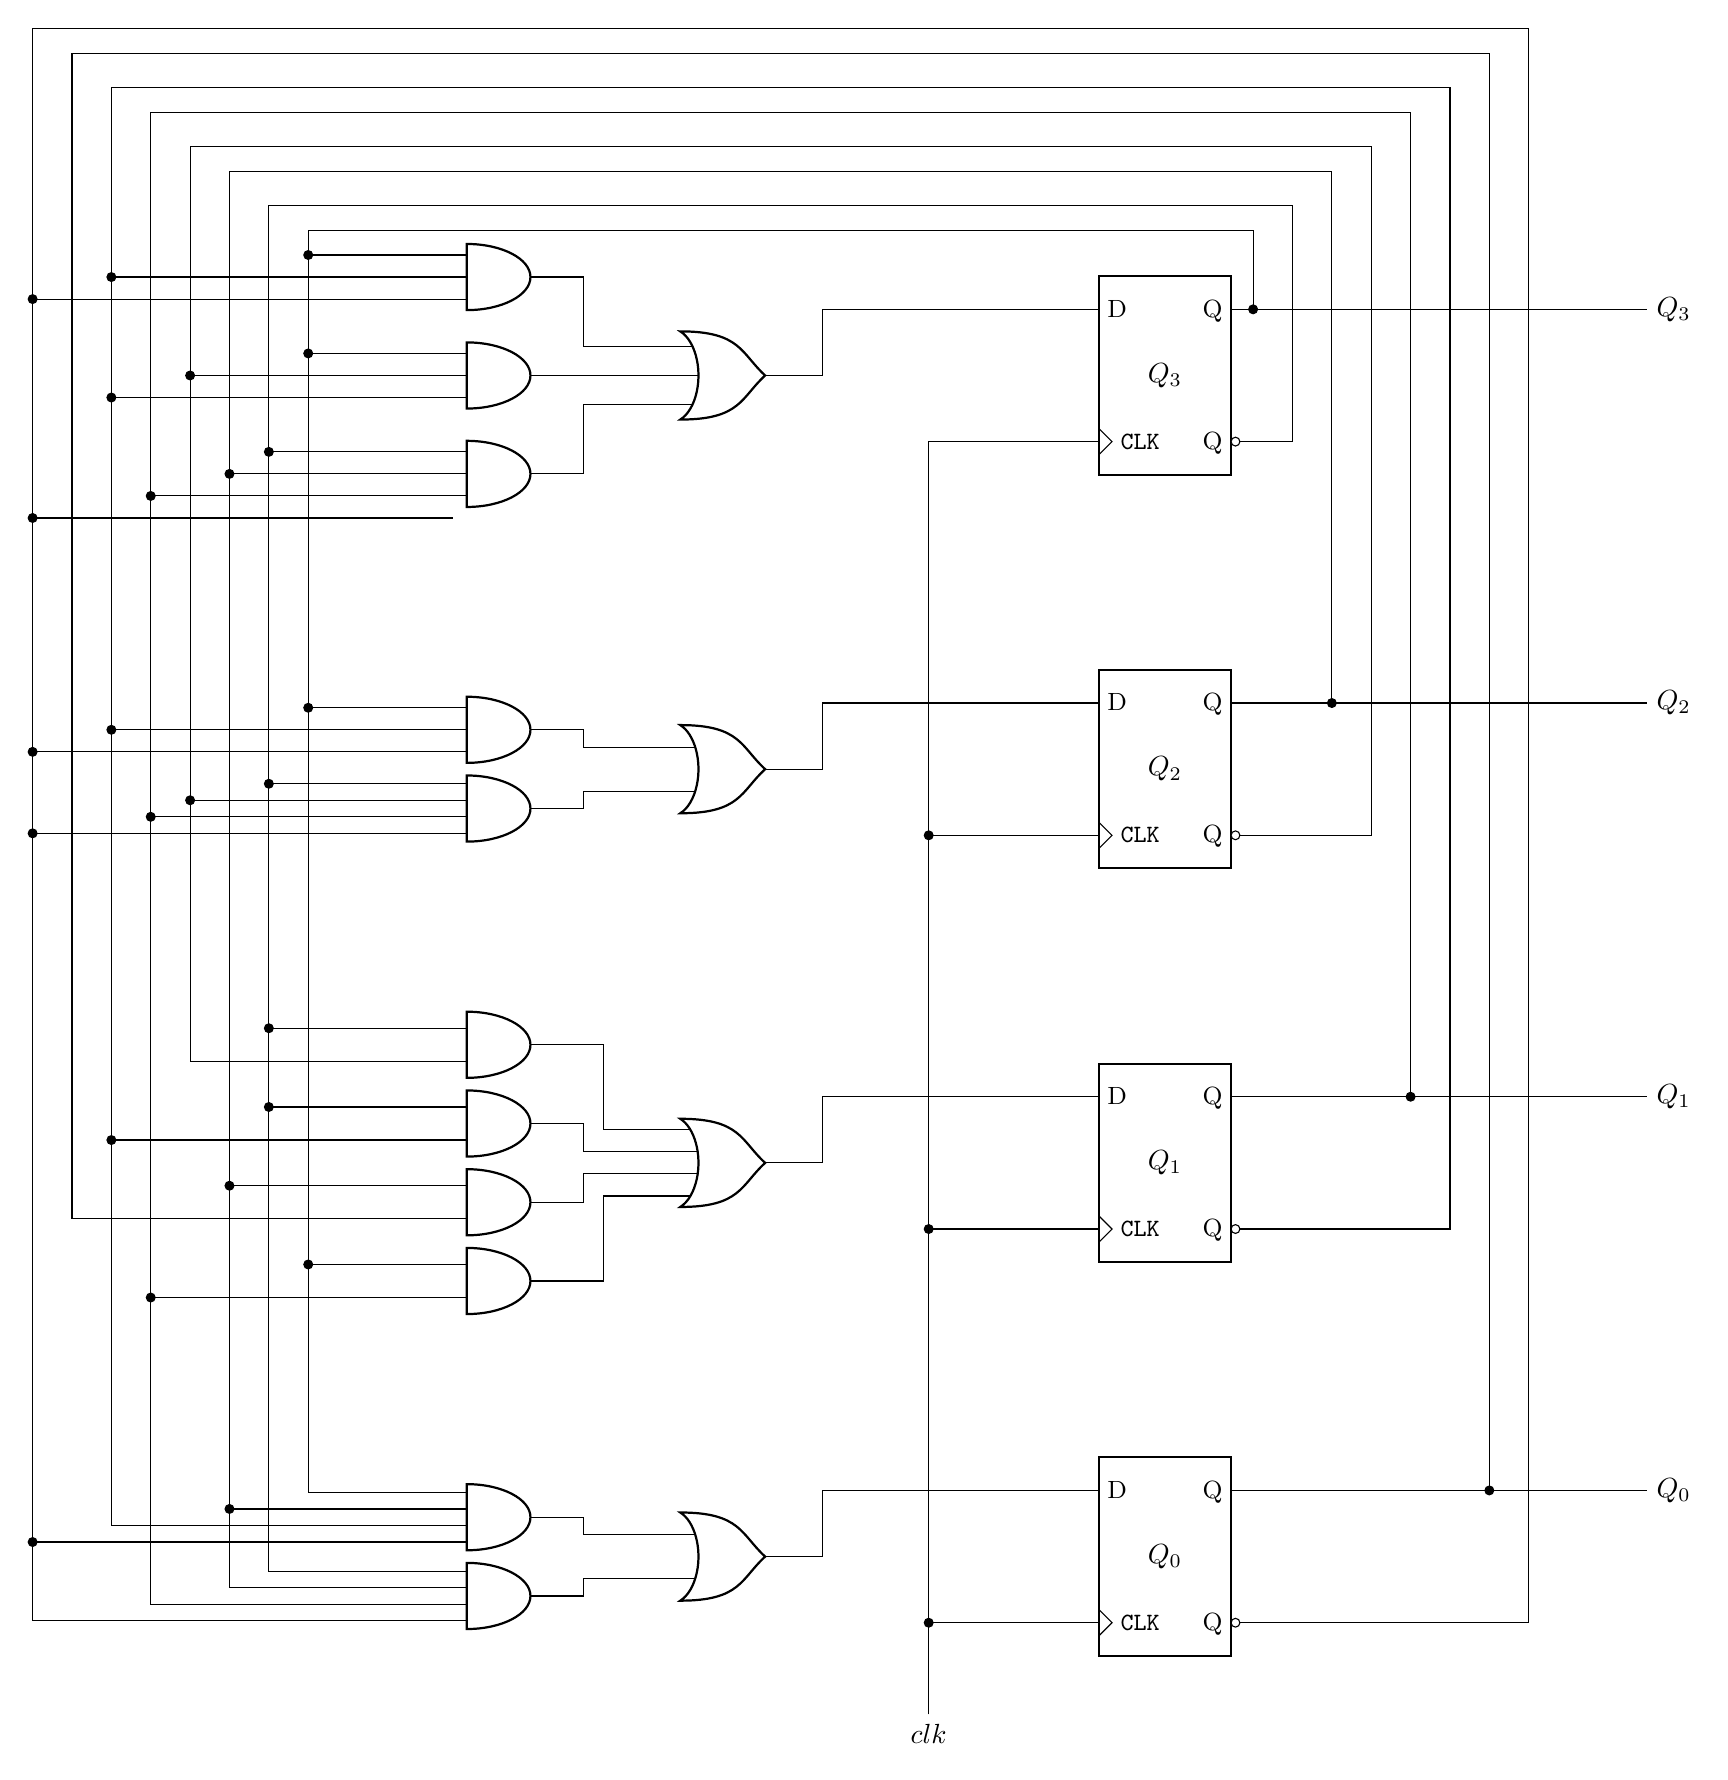
\begin{tikzpicture}
			\tikzset{myflipflop D/.style={flipflop,flipflop def={t1=D, t3={\texttt{CLK}}, t4=Q, t6=Q, n4=1, c3=1}}}
			\draw (8,0) node [myflipflop D] (DFF3) {$Q_3$};
			\draw (8,-5) node [myflipflop D] (DFF2) {$Q_2$};
			\draw (8,-10) node [myflipflop D] (DFF1) {$Q_1$};
			\draw (8,-15) node [myflipflop D] (DFF0) {$Q_0$};

			\draw (0,1.25) node [and port, number inputs=3, scale=0.75] (AND1) {};
			\draw (0,0) node [and port, number inputs=3, scale=0.75] (AND2) {};
			\draw (0,-1.25) node [and port, number inputs=3, scale=0.75] (AND3) {};
			\draw (3,0) node [or port, number inputs=3] (OR1) {};

			\draw (0,-4.5) node [and port, number inputs=3, scale=0.75] (AND4) {};
			\draw (0,-5.5) node [and port, number inputs=4, scale=0.75] (AND5) {};
			\draw (3,-5) node [or port] (OR2) {};

			\draw (0,-8.5) node [and port, scale=0.75] (AND6) {};
			\draw (0,-9.5) node [and port, scale=0.75] (AND7) {};
			\draw (0,-10.5) node [and port, scale=0.75] (AND8) {};
			\draw (0,-11.5) node [and port, scale=0.75] (AND9) {};
			\draw (3,-10) node [or port, number inputs=4] (OR3) {};

			\draw (0,-14.5) node [and port, number inputs=4, scale=0.75] (AND10) {};
			\draw (0,-15.5) node [and port, number inputs=4, scale=0.75] (AND11) {};
			\draw (3,-15) node [or port] (OR4) {};

			\draw (DFF3.pin 6) -- ++(0,1) -- ++(-12,0) coordinate (Q3) {};
			\draw (DFF3.pin 4) -| ++(0.5,3) -- ++(-13,0) coordinate (Q3') {};
			\draw (DFF2.pin 6) -| ++(1,6.75) -- ++(-14,0) coordinate (Q2) {};
			\draw (DFF2.pin 4) -| ++(1.5,8.75) -- ++(-15,0) coordinate (Q2') {};
			\draw (DFF1.pin 6) -| ++(2,12.5) -- ++(-16,0) coordinate (Q1) {};
			\draw (DFF1.pin 4) -| ++(2.5,14.5) -- ++(-17,0) coordinate (Q1') {};
			\draw (DFF0.pin 6) -| ++(3,18.25) -- ++(-18,0) coordinate (Q0) {};
			\draw (DFF0.pin 4) -| ++(3.5,20.25) -- ++(-19,0) coordinate (Q0') {};

			\draw (DFF3.pin 6) node [circ]{};
			\draw (DFF2.pin 6) ++ (1,0) node [circ]{};
			\draw (DFF1.pin 6) ++ (2,0) node [circ]{};
			\draw (DFF0.pin 6) ++ (3,0) node [circ]{};
 
			\draw (Q3) -- (Q3|-AND1.in 1) node[circ]{} -- (AND1.in 1);
			\draw (Q3) -- (Q3|-AND2.in 1) node[circ]{} -- (AND2.in 1);
			\draw (Q3) -- (Q3|-AND4.in 1) node[circ]{} -- (AND4.in 1);
			\draw (Q3) -- (Q3|-AND9.in 1) node[circ]{} -- (AND9.in 1);
			\draw (Q3) |- (AND10.in 1);

			\draw (Q3') -- (Q3'|-AND3.in 1) node[circ]{} -- (AND3.in 1);
			\draw (Q3') -- (Q3'|-AND5.in 1) node[circ]{} -- (AND5.in 1);
			\draw (Q3') -- (Q3'|-AND6.in 1) node[circ]{} -- (AND6.in 1);
			\draw (Q3') -- (Q3'|-AND7.in 1) node[circ]{} -- (AND7.in 1);
			\draw (Q3') |- (AND11.in 1);

			\draw (Q2) -- (Q2|-AND3.in 2) node[circ]{} -- (AND3.in 2);
			\draw (Q2) -- (Q2|-AND8.in 1) node[circ]{} -- (AND8.in 1);
			\draw (Q2) -- (Q2|-AND10.in 2) node[circ]{} -- (AND10.in 2);
			\draw (Q2) |- (AND11.in 2);

			\draw (Q2') -- (Q2'|-AND2.in 2) node[circ]{} -- (AND2.in 2);
			\draw (Q2') -- (Q2'|-AND5.in 2) node[circ]{} -- (AND5.in 2);
			\draw (Q2') |- (AND6.in 2);

			\draw (Q1) -- (Q1|-AND3.in 3) node[circ]{} -- (AND3.in 3);
			\draw (Q1) -- (Q1|-AND5.in 3) node[circ]{} -- (AND5.in 3);
			\draw (Q1) -- (Q1|-AND9.in 2) node[circ]{} -- (AND9.in 2);
			\draw (Q1) |- (AND11.in 3);

			\draw (Q1') -- (Q1'|-AND1.in 2) node[circ]{} -- (AND1.in 2);
			\draw (Q1') -- (Q1'|-AND2.in 3) node[circ]{} -- (AND2.in 3);
			\draw (Q1') -- (Q1'|-AND4.in 2) node[circ]{} -- (AND4.in 2);
			\draw (Q1') -- (Q1'|-AND7.in 2) node[circ]{} -- (AND7.in 2);
			\draw (Q1') |- (AND10.in 3);

			\draw (Q0) |- (AND8.in 2);

			\draw (Q0') -- (Q0'|-AND1.in 3) node[circ]{} -- (AND1.in 3);
			\draw (Q0') -- (Q0'|-AND3.in 4) node[circ]{} -- (AND3.in 4);
			\draw (Q0') -- (Q0'|-AND4.in 3) node[circ]{} -- (AND4.in 3);
			\draw (Q0') -- (Q0'|-AND5.in 4) node[circ]{} -- (AND5.in 4);
			\draw (Q0') -- (Q0'|-AND10.in 4) node[circ]{} -- (AND10.in 4);
			\draw (Q0') |- (AND11.in 4);

			\draw (AND1.out) -- ++(0.5,0) |- (OR1.in 1);
			\draw (AND2.out) -- ++(0.5,0) |- (OR1.in 2);
			\draw (AND3.out) -- ++(0.5,0) |- (OR1.in 3);
			\draw (OR1.out) -- ++(0.5,0) |- (DFF3.pin 1);

			\draw (AND4.out) -- ++(0.5,0) |- (OR2.in 1);
			\draw (AND5.out) -- ++(0.5,0) |- (OR2.in 2);
			\draw (OR2.out) -- ++(0.5,0) |- (DFF2.pin 1);

			\draw (AND6.out) -- ++(0.75,0) |- (OR3.in 1);
			\draw (AND7.out) -- ++(0.5,0) |- (OR3.in 2);
			\draw (AND8.out) -- ++(0.5,0) |- (OR3.in 3);
			\draw (AND9.out) -- ++(0.75,0) |- (OR3.in 4);
			\draw (OR3.out) -- ++(0.5,0) |- (DFF1.pin 1);

			\draw (AND10.out) -- ++(0.5,0) |- (OR4.in 1);
			\draw (AND11.out) -- ++(0.5,0) |- (OR4.in 2);
			\draw (OR4.out) -- ++(0.5,0) |- (DFF0.pin 1);

			\draw (5,-17) node [below] (clk) {$clk$};
			\draw (clk) |- (DFF3.pin 3);
			\draw (clk) -- (clk|-DFF2.pin 3) node[circ]{} -- (DFF2.pin 3);
			\draw (clk) -- (clk|-DFF1.pin 3) node[circ]{} -- (DFF1.pin 3);
			\draw (clk) -- (clk|-DFF0.pin 3) node[circ]{} -- (DFF0.pin 3);

			\draw (DFF3.pin 6) -- ++(5,0) node [right] {$Q_3$};
			\draw (DFF2.pin 6) -- ++(5,0) node [right] {$Q_2$};
			\draw (DFF1.pin 6) -- ++(5,0) node [right] {$Q_1$};
			\draw (DFF0.pin 6) -- ++(5,0) node [right] {$Q_0$};
		\end{tikzpicture}
	}
\end{center}

\newpage
\section*{4.}

\subsection*{With Don't Cares}

\textbf{State Table with TFF Inputs:}

\begin{center}
	\begin{tabular}{ccccccccc}
		\toprule
		\multicolumn{3}{c}{Current State} & \multicolumn{3}{c}{Next State} & \multicolumn{3}{c}{TFF Inputs} \\
		\cmidrule(lr){1-3} \cmidrule(lr){4-6} \cmidrule(lr){7-9}
		$Q_2$ & $Q_1$ & $Q_0$ & $Q_2^+$ & $Q_1^+$ & $Q_0^+$ & $T_2$ & $T_1$ & $T_0$ \\
		\midrule
		0 & 0 & 0 & 0 & 0 & 1 & 0 & 0 & 1 \\ 
        0 & 0 & 1 & 0 & 1 & 1 & 0 & 1 & 0 \\ 
        0 & 1 & 0 & x & x & x & x & x & x \\ 
        0 & 1 & 1 & 1 & 1 & 1 & 1 & 0 & 0 \\ 
        1 & 0 & 0 & 0 & 0 & 0 & 1 & 0 & 0 \\ 
        1 & 0 & 1 & x & x & x & x & x & x \\ 
        1 & 1 & 0 & 1 & 0 & 0 & 0 & 1 & 0 \\ 
        1 & 1 & 1 & 1 & 1 & 0 & 0 & 0 & 1 \\ 
		\bottomrule
	\end{tabular}
\end{center}

\textbf{Karnaugh Maps:}

\begin{figure}[H]
	\begin{minipage}{0.5\linewidth}
		\centering
		\begin{karnaugh-map}(label=corner)[4][2][1][$Q_1Q_0$][$Q_2$]
			\minterms{3,4}
			\maxterms{0,1,6,7}
			\autoterms[X]
			\implicant{3}{2}
			\implicant{4}{5}
		\end{karnaugh-map}
		\caption*{$T_2$}
	\end{minipage}
	\begin{minipage}{0.5\linewidth}
		\centering
		\begin{karnaugh-map}(label=corner)[4][2][1][$Q_1Q_0$][$Q_2$]
			\minterms{1,6}
			\maxterms{0,3,4,7}
			\autoterms[X]
			\implicant{1}{5}
			\implicant{2}{6}
		\end{karnaugh-map}
		\caption*{$T_1$}
	\end{minipage}
\end{figure}

\begin{figure}[H]
	\begin{minipage}{0.5\linewidth}
		\centering
		\begin{karnaugh-map}(label=corner)[4][2][1][$Q_1Q_0$][$Q_2$]
			\minterms{0,7}
			\maxterms{1,3,4,6}
			\autoterms[X]
			\implicant{5}{7}
			\implicantedge{0}{0}{2}{2}
		\end{karnaugh-map}
		\caption*{$T_0$}
	\end{minipage}
\end{figure}

\textbf{Simplified Boolean Expression:}

\begin{align*}
	T_2 =& Q_2'Q_1 + Q_2Q_1' \\
	T_1 =& Q_1'Q_0 + Q_1Q_0' \\
	T_0 =& Q_2'Q_0' + Q_2Q_0
\end{align*}

\newpage
In this case, the actual state table is:
\begin{center}
	\begin{tabular}{ccccccccc}
		\toprule
		\multicolumn{3}{c}{Current State} & \multicolumn{3}{c}{Next State} & \multicolumn{3}{c}{TFF Inputs} \\
		\cmidrule(lr){1-3} \cmidrule(lr){4-6} \cmidrule(lr){7-9}
		$Q_2$ & $Q_1$ & $Q_0$ & $Q_2^+$ & $Q_1^+$ & $Q_0^+$ & $T_2$ & $T_1$ & $T_0$ \\
		\midrule
		0 & 0 & 0 & 0 & 0 & 1 & 0 & 0 & 1 \\ 
        0 & 0 & 1 & 0 & 1 & 1 & 0 & 1 & 0 \\ 
		\rowcolor{red!20}
        0 & 1 & 0 & 1 & 0 & 1 & 1 & 1 & 1 \\ 
        0 & 1 & 1 & 1 & 1 & 1 & 1 & 0 & 0 \\ 
        1 & 0 & 0 & 0 & 0 & 0 & 1 & 0 & 0 \\ 
		\rowcolor{red!20}
        1 & 0 & 1 & 0 & 1 & 0 & 1 & 1 & 1 \\ 
        1 & 1 & 0 & 1 & 0 & 0 & 0 & 1 & 0 \\ 
        1 & 1 & 1 & 1 & 1 & 0 & 0 & 0 & 1 \\ 
		\bottomrule
	\end{tabular}
\end{center}

As shown in the state table, the states with don't cares form a loop.
Thus, the counter may not work properly.

\subsection*{Without Don't Cares}

We can force the unused states go to the 000 state.

\textbf{State Table with TFF Inputs:}

\begin{center}
	\begin{tabular}{ccccccccc}
		\toprule
		\multicolumn{3}{c}{Current State} & \multicolumn{3}{c}{Next State} & \multicolumn{3}{c}{TFF Inputs} \\
		\cmidrule(lr){1-3} \cmidrule(lr){4-6} \cmidrule(lr){7-9}
		$Q_2$ & $Q_1$ & $Q_0$ & $Q_2^+$ & $Q_1^+$ & $Q_0^+$ & $T_2$ & $T_1$ & $T_0$ \\
		\midrule
		0 & 0 & 0 & 0 & 0 & 1 & 0 & 0 & 1 \\ 
        0 & 0 & 1 & 0 & 1 & 1 & 0 & 1 & 0 \\ 
        0 & 1 & 0 & 0 & 0 & 0 & 0 & 1 & 0 \\ 
        0 & 1 & 1 & 1 & 1 & 1 & 1 & 0 & 0 \\ 
        1 & 0 & 0 & 0 & 0 & 0 & 1 & 0 & 0 \\ 
        1 & 0 & 1 & 0 & 0 & 0 & 1 & 0 & 1 \\ 
        1 & 1 & 0 & 1 & 0 & 0 & 0 & 1 & 0 \\ 
        1 & 1 & 1 & 1 & 1 & 0 & 0 & 0 & 1 \\ 
		\bottomrule
	\end{tabular}
\end{center}

\textbf{Karnaugh Maps:}

\begin{figure}[H]
	\begin{minipage}{0.5\linewidth}
		\centering
		\begin{karnaugh-map}(label=corner)[4][2][1][$Q_1Q_0$][$Q_2$]
			\minterms{3,4,5}
			\maxterms{0,1,2,6,7}
			\implicant{4}{5}
			\implicant{3}{3}
		\end{karnaugh-map}
		\caption*{$T_2$}
	\end{minipage}
	\begin{minipage}{0.5\linewidth}
		\centering
		\begin{karnaugh-map}(label=corner)[4][2][1][$Q_1Q_0$][$Q_2$]
			\minterms{1,2,6}
			\maxterms{0,3,4,5,7}
			\implicant{2}{6}
			\implicant{1}{1}
		\end{karnaugh-map}
		\caption*{$T_1$}
	\end{minipage}
\end{figure}

\begin{figure}[H]
	\begin{minipage}{0.5\linewidth}
		\centering
		\begin{karnaugh-map}(label=corner)[4][2][1][$Q_1Q_0$][$Q_2$]
			\minterms{0,5,7}
			\maxterms{1,2,3,4,6}
			\implicant{5}{7}
			\implicant{0}{0}
		\end{karnaugh-map}
		\caption*{$T_0$}
	\end{minipage}
\end{figure}

\textbf{Simplified Boolean Expression:}

\begin{align*}
	T_2 =& Q_2Q_1' + Q_2'Q_1Q_0 \\
	T_1 =& Q_1Q_0' + Q_2'Q_1'Q_0 \\
	T_0 =& Q_2Q_0 + Q_2'Q_1'Q_0'
\end{align*}
\end{document}